\scanpage{68}
% @ full sheet, long cancellation strokes | drawing
\figure{\begin{tikzpicture}[x=.41cm,y=.41cm]
\draw[thin] (1.1,7.8) .. controls (1.0,7.1) and (2.0,3.6) .. (3.1,.3);
\draw[thin] (4.6,8.7) .. controls (4.5,6.7) and (5.9,2.2) .. (6.0,.5);
\draw[thin] (7.0,9.0) .. controls (6.45,7.4) and (7.2,3.35) .. (7.8,1.55);
\end{tikzpicture}}
% @ top left | display
\[
 \Sigma^1 X
\]
% @ top centre, pair and arrow | diagram
\diagram{\begin{tikzcd}[ampersand replacement=\&,row sep=tiny,column sep=tiny]
 \& (X,e)\arrow[dl]\\ e \&
\end{tikzcd}}

% @ upper left, double cone with hatched section | drawing
\figure{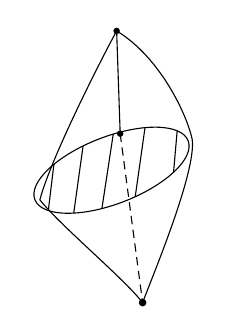
\begin{tikzpicture}[scale=.75,line join=round]
\coordinate (t) at (.04,2.48); \coordinate (b) at (.48,-2.12);
\draw (t) .. controls (.77,2.04) and (1.23,1.07) .. (1.32,.64)
 .. controls (1.39,.09) and (.64,-1.69) .. (b)
 .. controls (.14,-1.69) and (-.91,-.82) .. (-1.26,-.38)
 .. controls (-1.07,.34) and (-.20,2.04) .. (t);
\begin{scope}[rotate=21]
\draw (0,.13) ellipse (1.39 and .57);
\begin{scope}
\clip (0,.13) ellipse (1.39 and .57);
\draw (-1.39,-.40)--(-.75,.81) (-.98,-.54)--(-.19,.89) (-.46,-.55)--(.36,.89) (.16,-.53)--(.96,.91) (.87,-.48)--(1.46,.73);
\end{scope}\end{scope}
\draw (t)--(.10,.74);\draw[densely dashed] (.10,.74)--(b);
\fill (t) circle (.055) (.10,.74) circle (.055) (b) circle (.065);
\end{tikzpicture}}

% @ upper centre, open diamond | diagram
\diagram{\begin{tikzcd}[ampersand replacement=\&,row sep=tiny,column sep=tiny]
 \& {}\arrow[dl,no head]\arrow[dr,no head] \&\\
 \bullet \& \& \cdot\\
 \& {}\arrow[ul,no head]\arrow[ur,no head] \&
\end{tikzcd}}

% @ centre left | diagram
\diagram{\begin{tikzcd}[ampersand replacement=\&,row sep=tiny]
 \&\deleted{X\times Y}\arrow[dl]\\ {} \&
\end{tikzcd}}

% @ centre, small pair | display
\[
 \deleted{\unsure{x,y|x,y'}}
\]

% @ centre right, four-vertex diagram | diagram
\diagram{\begin{tikzcd}[ampersand replacement=\&,row sep=small,column sep=small]
 \& X_0\arrow[dl]\arrow[dr,no head] \&\\
 X_1\arrow[dr] \& \& X_2\arrow[dl]\\
 \& X_3 \&
\end{tikzcd}}

% @ lower left | diagram
\diagram{\begin{tikzcd}[ampersand replacement=\&]
 X\arrow[r] \& \deleted{X\times I}
\end{tikzcd}}

% @ lower right | display
\[
 \deleted{x_0\times I}
\]
% archive sheet number: 67
